% Options for packages loaded elsewhere
\PassOptionsToPackage{unicode}{hyperref}
\PassOptionsToPackage{hyphens}{url}
%
\documentclass[
  ignorenonframetext,
]{beamer}
\usepackage{pgfpages}
\setbeamertemplate{caption}[numbered]
\setbeamertemplate{caption label separator}{: }
\setbeamercolor{caption name}{fg=normal text.fg}
\beamertemplatenavigationsymbolsempty
% Prevent slide breaks in the middle of a paragraph
\widowpenalties 1 10000
\raggedbottom
\setbeamertemplate{part page}{
  \centering
  \begin{beamercolorbox}[sep=16pt,center]{part title}
    \usebeamerfont{part title}\insertpart\par
  \end{beamercolorbox}
}
\setbeamertemplate{section page}{
  \centering
  \begin{beamercolorbox}[sep=12pt,center]{part title}
    \usebeamerfont{section title}\insertsection\par
  \end{beamercolorbox}
}
\setbeamertemplate{subsection page}{
  \centering
  \begin{beamercolorbox}[sep=8pt,center]{part title}
    \usebeamerfont{subsection title}\insertsubsection\par
  \end{beamercolorbox}
}
\AtBeginPart{
  \frame{\partpage}
}
\AtBeginSection{
  \ifbibliography
  \else
    \frame{\sectionpage}
  \fi
}
\AtBeginSubsection{
  \frame{\subsectionpage}
}
\usepackage{lmodern}
\usepackage{amssymb,amsmath}
\usepackage{ifxetex,ifluatex}
\ifnum 0\ifxetex 1\fi\ifluatex 1\fi=0 % if pdftex
  \usepackage[T1]{fontenc}
  \usepackage[utf8]{inputenc}
  \usepackage{textcomp} % provide euro and other symbols
\else % if luatex or xetex
  \usepackage{unicode-math}
  \defaultfontfeatures{Scale=MatchLowercase}
  \defaultfontfeatures[\rmfamily]{Ligatures=TeX,Scale=1}
\fi
% Use upquote if available, for straight quotes in verbatim environments
\IfFileExists{upquote.sty}{\usepackage{upquote}}{}
\IfFileExists{microtype.sty}{% use microtype if available
  \usepackage[]{microtype}
  \UseMicrotypeSet[protrusion]{basicmath} % disable protrusion for tt fonts
}{}
\makeatletter
\@ifundefined{KOMAClassName}{% if non-KOMA class
  \IfFileExists{parskip.sty}{%
    \usepackage{parskip}
  }{% else
    \setlength{\parindent}{0pt}
    \setlength{\parskip}{6pt plus 2pt minus 1pt}}
}{% if KOMA class
  \KOMAoptions{parskip=half}}
\makeatother
\usepackage{xcolor}
\IfFileExists{xurl.sty}{\usepackage{xurl}}{} % add URL line breaks if available
\IfFileExists{bookmark.sty}{\usepackage{bookmark}}{\usepackage{hyperref}}
\hypersetup{
  pdftitle={MQE: Economic Inference from Data: Module 4: Randomized Control Trials},
  pdfauthor={Claire Duquennois},
  hidelinks,
  pdfcreator={LaTeX via pandoc}}
\urlstyle{same} % disable monospaced font for URLs
\newif\ifbibliography
\usepackage{color}
\usepackage{fancyvrb}
\newcommand{\VerbBar}{|}
\newcommand{\VERB}{\Verb[commandchars=\\\{\}]}
\DefineVerbatimEnvironment{Highlighting}{Verbatim}{commandchars=\\\{\}}
% Add ',fontsize=\small' for more characters per line
\usepackage{framed}
\definecolor{shadecolor}{RGB}{248,248,248}
\newenvironment{Shaded}{\begin{snugshade}}{\end{snugshade}}
\newcommand{\AlertTok}[1]{\textcolor[rgb]{0.94,0.16,0.16}{#1}}
\newcommand{\AnnotationTok}[1]{\textcolor[rgb]{0.56,0.35,0.01}{\textbf{\textit{#1}}}}
\newcommand{\AttributeTok}[1]{\textcolor[rgb]{0.77,0.63,0.00}{#1}}
\newcommand{\BaseNTok}[1]{\textcolor[rgb]{0.00,0.00,0.81}{#1}}
\newcommand{\BuiltInTok}[1]{#1}
\newcommand{\CharTok}[1]{\textcolor[rgb]{0.31,0.60,0.02}{#1}}
\newcommand{\CommentTok}[1]{\textcolor[rgb]{0.56,0.35,0.01}{\textit{#1}}}
\newcommand{\CommentVarTok}[1]{\textcolor[rgb]{0.56,0.35,0.01}{\textbf{\textit{#1}}}}
\newcommand{\ConstantTok}[1]{\textcolor[rgb]{0.00,0.00,0.00}{#1}}
\newcommand{\ControlFlowTok}[1]{\textcolor[rgb]{0.13,0.29,0.53}{\textbf{#1}}}
\newcommand{\DataTypeTok}[1]{\textcolor[rgb]{0.13,0.29,0.53}{#1}}
\newcommand{\DecValTok}[1]{\textcolor[rgb]{0.00,0.00,0.81}{#1}}
\newcommand{\DocumentationTok}[1]{\textcolor[rgb]{0.56,0.35,0.01}{\textbf{\textit{#1}}}}
\newcommand{\ErrorTok}[1]{\textcolor[rgb]{0.64,0.00,0.00}{\textbf{#1}}}
\newcommand{\ExtensionTok}[1]{#1}
\newcommand{\FloatTok}[1]{\textcolor[rgb]{0.00,0.00,0.81}{#1}}
\newcommand{\FunctionTok}[1]{\textcolor[rgb]{0.00,0.00,0.00}{#1}}
\newcommand{\ImportTok}[1]{#1}
\newcommand{\InformationTok}[1]{\textcolor[rgb]{0.56,0.35,0.01}{\textbf{\textit{#1}}}}
\newcommand{\KeywordTok}[1]{\textcolor[rgb]{0.13,0.29,0.53}{\textbf{#1}}}
\newcommand{\NormalTok}[1]{#1}
\newcommand{\OperatorTok}[1]{\textcolor[rgb]{0.81,0.36,0.00}{\textbf{#1}}}
\newcommand{\OtherTok}[1]{\textcolor[rgb]{0.56,0.35,0.01}{#1}}
\newcommand{\PreprocessorTok}[1]{\textcolor[rgb]{0.56,0.35,0.01}{\textit{#1}}}
\newcommand{\RegionMarkerTok}[1]{#1}
\newcommand{\SpecialCharTok}[1]{\textcolor[rgb]{0.00,0.00,0.00}{#1}}
\newcommand{\SpecialStringTok}[1]{\textcolor[rgb]{0.31,0.60,0.02}{#1}}
\newcommand{\StringTok}[1]{\textcolor[rgb]{0.31,0.60,0.02}{#1}}
\newcommand{\VariableTok}[1]{\textcolor[rgb]{0.00,0.00,0.00}{#1}}
\newcommand{\VerbatimStringTok}[1]{\textcolor[rgb]{0.31,0.60,0.02}{#1}}
\newcommand{\WarningTok}[1]{\textcolor[rgb]{0.56,0.35,0.01}{\textbf{\textit{#1}}}}
\usepackage{longtable,booktabs}
\usepackage{caption}
% Make caption package work with longtable
\makeatletter
\def\fnum@table{\tablename~\thetable}
\makeatother
\usepackage{graphicx}
\makeatletter
\def\maxwidth{\ifdim\Gin@nat@width>\linewidth\linewidth\else\Gin@nat@width\fi}
\def\maxheight{\ifdim\Gin@nat@height>\textheight\textheight\else\Gin@nat@height\fi}
\makeatother
% Scale images if necessary, so that they will not overflow the page
% margins by default, and it is still possible to overwrite the defaults
% using explicit options in \includegraphics[width, height, ...]{}
\setkeys{Gin}{width=\maxwidth,height=\maxheight,keepaspectratio}
% Set default figure placement to htbp
\makeatletter
\def\fps@figure{htbp}
\makeatother
\setlength{\emergencystretch}{3em} % prevent overfull lines
\providecommand{\tightlist}{%
  \setlength{\itemsep}{0pt}\setlength{\parskip}{0pt}}
\setcounter{secnumdepth}{-\maxdimen} % remove section numbering

\title{MQE: Economic Inference from Data:\\
Module 4: Randomized Control Trials}
\author{Claire Duquennois}
\date{6/9/2020}

\begin{document}
\frame{\titlepage}

\begin{frame}{Causal Inference with non-random assignment:}
\protect\hypertarget{causal-inference-with-non-random-assignment}{}
Randomizing treatment is not always possible:

\begin{itemize}
\item
  the program or policy has already happened
\item
  randomization in unfeasible
\item
  randomizing treatment would be unethical (ex: randomizing exposure to
  pollutants)
\end{itemize}
\end{frame}

\begin{frame}{Causal Inference with non-random assignment:}
\protect\hypertarget{causal-inference-with-non-random-assignment-1}{}
With no randomized control trial we have to assume that the treatment
was not randomly assigned:

\begin{itemize}
\item
  treatment will depend on observable and/or unobservable
  characteristics
\item
  their are important differences between our treated and untreated
  units that we cannot control for
\item
  Leaving these variables out in the error term will cause OVB.
\end{itemize}

Differences-in-differences is a way of getting around non-random
assignment of a treatment.
\end{frame}

\begin{frame}{DID: Example and intuition\footnote<.->{This section is
  borrowed from scunning.com}}
\protect\hypertarget{did-example-and-intuition}{}
2002: Craigslist opens a new section called ``erotic services'' in San
Francisco:

\begin{itemize}
\item
  mostly used by sex workers to advertise and solicit clients.
\item
  Sex workers claimed it made them safer, because they could solicit
  indoors from their computers and learn more about the men contacting
  them.
\item
  Activists and law enforcement worried that it was facilitating sex
  trafficking and increasing violence against women.
\end{itemize}

Which was it? Was erotic services (ERS) making women safer, or was it
placing them in harm's way?
\end{frame}

\begin{frame}{SOS Empiricist!}
\protect\hypertarget{sos-empiricist}{}
This is an empirical question: What is the effect of ERS on female
safety?

\begin{itemize}
\item
  The fundamental problem of causal inference strikes again!
\item
  We can't know what effect it had because we are missing the data for
  the counterfactual:
\end{itemize}

\[
E[\tau]=E[\underbrace{Y_{SF,2003}(D_{SF,2003}=1)}_\text{observed}]-E[\underbrace{Y_{SF,2003}(D_{SF,2003}=0)}_\text{unobserved}]
\]

In 2003 only the first occurs, and the second is a counterfactual. So
how do we proceed?
\end{frame}

\begin{frame}{Diff-in-Diff to the rescue:}
\protect\hypertarget{diff-in-diff-to-the-rescue}{}
The standard differences-in-differences strategy (DiD):

\begin{itemize}
\item
  Define the intervention, \(D\)= the availability of the Craigslist ERS
  webpage.
\item
  We want to know the causal effect, \(\tau\) of \(D\) on \(Y\)= female
  murders.
\end{itemize}

Can we just compare SF murders in, say, 2003 with some other city, like
Pittsburgh?
\end{frame}

\begin{frame}{Differencing A:}
\protect\hypertarget{differencing-a}{}
\begin{longtable}[]{@{}ll@{}}
\toprule
\ldots.City\ldots. &
\ldots\ldots\ldots..Outcome\ldots\ldots\ldots\ldots.\tabularnewline
\midrule
\endhead
San Francisco & \(Y_{SF,2003}=\alpha_{SF}+\tau\)\tabularnewline
Pittsburgh & \(Y_{P,2003}=\alpha_{P}\)\tabularnewline
\bottomrule
\end{longtable}

\begin{itemize}
\item
  \(\alpha_{SF}\) is a San Francisco fixed effect
\item
  \(\alpha_P\) is a Pittsburgh fixed effect.
\end{itemize}

If make a simple comparison between Pittsburgh and SF:

\[
\tilde{\tau}=Y_{SF,2003}-Y_{P,2003}=\alpha_{SF}+\tau-\alpha_{P}.
\]
\end{frame}

\begin{frame}{Differencing A:}
\protect\hypertarget{differencing-a-1}{}
The simple difference is biased because of the difference in the
underlying murder rates between the two cities:

\[
\tilde{\tau}-\tau=\alpha_{SF}-\alpha_{P}. 
\]
\end{frame}

\begin{frame}{Differencing B:}
\protect\hypertarget{differencing-b}{}
What if we compare SF to itself? Say in 2003 to 2001?

\begin{longtable}[]{@{}ccc@{}}
\toprule
\ldots..City\ldots. & ..Time.. &
\ldots\ldots\ldots.Outcome\ldots\ldots\ldots\ldots.\tabularnewline
\midrule
\endhead
San Francisco & Before & \(Y_{SF,2001}=\alpha_{SF}\)\tabularnewline
& After & \(Y_{SF,2003}=\alpha_{SF}+\lambda_{03}+\tau\)\tabularnewline
\bottomrule
\end{longtable}

Again, this doesn't lead to an unbiased estimate of \(\tau\) since: \[
\tilde{\tau}=\alpha_{SF}+\lambda_{03}+\tau-\alpha_{SF}=\lambda_{03}+\tau
\]

We eliminated the city fixed effect but not the changes in the murder
rate over time which will bias my estimate: \[
\tilde{\tau}-\tau=\lambda_{03}
\] \textbf{How can I identify and control for these time effects?}
\end{frame}

\begin{frame}{Differencing A+B= Diff-in-Diff}
\protect\hypertarget{differencing-ab-diff-in-diff}{}
Combining the two approaches to eliminate both the city effects and the
time effects:

\begin{longtable}[]{@{}lllll@{}}
\toprule
\ldots City\ldots{} & ..Time.. & \ldots\ldots..Outcome\ldots\ldots.. &
1st Diff & 2nd Diff\tabularnewline
\midrule
\endhead
SF & Before & \(Y_{SF,2001}=\alpha_{SF}\) & &\tabularnewline
& After & \(Y_{SF,2003}=\alpha_{SF}+\lambda_{03}+\tau\) &
\(\lambda_{03}+\tau\) &\tabularnewline
& & & & \(\tau\)\tabularnewline
Pittsburgh & Before & \(Y_{P,2001}=\alpha_{P}\) & &\tabularnewline
& After & \(Y_{P,2003}=\alpha_{P}+\lambda_{03}\) & \(\lambda_{03}\)
&\tabularnewline
\bottomrule
\end{longtable}
\end{frame}

\begin{frame}{The idea}
\protect\hypertarget{the-idea}{}
Sometimes treatment and control group outcomes move in parallel in the
absence of treatment.

When they do, the divergence of a post-treatment path from the trend
established by a comparison group may signal a treatment effect.
\end{frame}

\begin{frame}{The mechanics}
\protect\hypertarget{the-mechanics}{}
Difference-in-differences can be implemented as follows:

\begin{enumerate}
[1)]
\tightlist
\item
  Compute the difference in the mean outcome variable \(Y\) in the post
  treatment period \((t=1)\) and the before treatment period \((t=0)\)
  for the control group \(C\):
\end{enumerate}

\[
\bar{Y}_{C,1}-\bar{Y}_{C,0}=\Delta \bar{Y}_C
\]

\(\Rightarrow\) allows us to cancel out the control group fixed effect
and identify the time fixed effect since \[
\bar{Y}_{C,1}-\bar{Y}_{C,0}=\alpha_C+\lambda_1-\alpha_C=\lambda_1=\Delta \bar{Y}_C
\]
\end{frame}

\begin{frame}{The mechanics}
\protect\hypertarget{the-mechanics-1}{}
\begin{enumerate}
[1)]
\setcounter{enumi}{1}
\tightlist
\item
  Compute the difference in the mean outcome variable \(Y\) in the post
  treatment period \((t=1)\) and the before treatment period \((t=0)\)
  for the treated group \(T\):
\end{enumerate}

\[
\bar{Y}_{T,1}-\bar{Y}_{T,0}=\Delta \bar{Y}_T
\] which allows us to cancel out the treated group fixed effect \[
\bar{Y}_{T,1}-\bar{Y}_{T,0}=\alpha_T+\lambda_1+\tau-\alpha_T=\lambda_1+\tau=\Delta \bar{Y}_T
\]
\end{frame}

\begin{frame}{The mechanics}
\protect\hypertarget{the-mechanics-2}{}
\begin{enumerate}
[1)]
\setcounter{enumi}{2}
\tightlist
\item
  Treatment impact is then measured by the difference-in-differences:
\end{enumerate}

\[
(\bar{Y}_{T,1}-\bar{Y}_{T,0})-(\bar{Y}_{C,1}-\bar{Y}_{C,0})=(\Delta \bar{Y}_T-\Delta \bar{Y}_C)
\] since by comparing the differences we can cancel out the time fixed
effect and isolate the treatment effect of interest:

\[
\Delta \bar{Y}_T-\Delta \bar{Y}_C=\lambda_1+\tau-\lambda_1=\tau
\]
\end{frame}

\begin{frame}{DID Regressions:}
\protect\hypertarget{did-regressions}{}
This can be done in a regression framework:

\[
Y_{it}=\beta_0+\beta_1 Post_t+\beta_2 GetsTreat_i+\beta_3 Post_t\times GetsTreat_i+u_{it}
\]

\begin{itemize}
\item
  \(Post_t\) is an indicator for the post treatment period,
\item
  \(GetsTreat_i\) is an indicator for observations in the treatment
  group that eventually gets treated.
\end{itemize}
\end{frame}

\begin{frame}{DID Regressions:}
\protect\hypertarget{did-regressions-1}{}
\(\beta_3\) is the difference-in-differences estimator:

\begin{itemize}
\tightlist
\item
  estimates the differential impact of being in the post treatment
  period if you are in the treated group since
\end{itemize}

\small

\[
\begin{aligned}
E[Y_{C,1}]-E[Y_{C,0}]&=(\beta_0+\beta_1)-(\beta_0)=\beta_1\\
E[Y_{T,1}]-E[Y_{T,0}]&=(\beta_0+\beta_1+\beta_2+\beta_3)-(\beta_0+\beta_2)=\beta_1+\beta_3\\
\end{aligned}
\]

\[
(E[Y_{T,1}]-E[Y_{T,0}])-(E[Y_{C,1}]-E[Y_{C,0}])=\beta_3
\]
\end{frame}

\begin{frame}{A simulation:}
\protect\hypertarget{a-simulation}{}
Suppose you are a principal of a school:

\begin{itemize}
\item
  ten 4th grade classrooms of 30 students each.
\item
  Starting in 2001 school year, teachers can enroll their class in the
  scholastic book club
\item
  4 of your fourth grade teachers opted to enroll.
\end{itemize}

You are interested in estimating the effect of participation in the book
club on 4th grade reading scores.
\end{frame}

\begin{frame}[fragile]{A simulation:}
\protect\hypertarget{a-simulation-1}{}
\tiny

\begin{Shaded}
\begin{Highlighting}[]
\KeywordTok{set.seed}\NormalTok{(}\DecValTok{6000}\NormalTok{)}
\NormalTok{scores\textless{}{-}}\KeywordTok{as.data.frame}\NormalTok{(}\KeywordTok{rep}\NormalTok{(}\KeywordTok{c}\NormalTok{(}\DecValTok{1}\NormalTok{,}\DecValTok{2}\NormalTok{,}\DecValTok{3}\NormalTok{,}\DecValTok{4}\NormalTok{,}\DecValTok{5}\NormalTok{,}\DecValTok{6}\NormalTok{,}\DecValTok{7}\NormalTok{,}\DecValTok{8}\NormalTok{,}\DecValTok{9}\NormalTok{,}\DecValTok{10}\NormalTok{),}\DataTypeTok{times=}\DecValTok{30}\NormalTok{))}
\KeywordTok{names}\NormalTok{(scores)\textless{}{-}}\KeywordTok{c}\NormalTok{(}\StringTok{"class"}\NormalTok{)}
\NormalTok{scores \textless{}{-}}\StringTok{ }\NormalTok{fastDummies}\OperatorTok{::}\KeywordTok{dummy\_cols}\NormalTok{(scores, }\DataTypeTok{select\_columns =} \StringTok{"class"}\NormalTok{)}

\NormalTok{scores}\OperatorTok{$}\NormalTok{error\textless{}{-}}\KeywordTok{rnorm}\NormalTok{(}\DecValTok{300}\NormalTok{, }\DataTypeTok{mean=}\DecValTok{0}\NormalTok{, }\DataTypeTok{sd=}\DecValTok{10}\NormalTok{)}

\CommentTok{\#suppose teachers in the better performing classes (classes, 7,8,9,10) select to participate in the book club program}
\NormalTok{scores}\OperatorTok{$}\NormalTok{treat\textless{}{-}}\DecValTok{0}
\NormalTok{scores}\OperatorTok{$}\NormalTok{treat[scores}\OperatorTok{$}\NormalTok{class}\OperatorTok{\%in\%}\KeywordTok{c}\NormalTok{(}\DecValTok{7}\NormalTok{,}\DecValTok{8}\NormalTok{,}\DecValTok{9}\NormalTok{,}\DecValTok{10}\NormalTok{)]\textless{}{-}}\DecValTok{1}

\NormalTok{tau\textless{}{-}}\DecValTok{10}

\CommentTok{\#the data generating process}
\NormalTok{scores}\OperatorTok{$}\NormalTok{read4\textless{}{-}(}\DecValTok{85}\OperatorTok{+}\NormalTok{tau}\OperatorTok{*}\NormalTok{scores}\OperatorTok{$}\NormalTok{treat}
               \OperatorTok{+}\NormalTok{(}\OperatorTok{{-}}\DecValTok{10}\NormalTok{)}\OperatorTok{*}\NormalTok{scores}\OperatorTok{$}\NormalTok{class\_}\DecValTok{1}\OperatorTok{+}\NormalTok{(}\OperatorTok{{-}}\DecValTok{15}\NormalTok{)}\OperatorTok{*}\NormalTok{scores}\OperatorTok{$}\NormalTok{class\_}\DecValTok{2}\OperatorTok{+}\NormalTok{(}\OperatorTok{{-}}\DecValTok{5}\NormalTok{)}\OperatorTok{*}\NormalTok{scores}\OperatorTok{$}\NormalTok{class\_}\DecValTok{3}
               \OperatorTok{+}\NormalTok{(}\OperatorTok{{-}}\DecValTok{8}\NormalTok{)}\OperatorTok{*}\NormalTok{scores}\OperatorTok{$}\NormalTok{class\_}\DecValTok{4}\OperatorTok{+}\NormalTok{(}\OperatorTok{{-}}\DecValTok{3}\NormalTok{)}\OperatorTok{*}\NormalTok{scores}\OperatorTok{$}\NormalTok{class\_}\DecValTok{5}\OperatorTok{+}\NormalTok{(}\DecValTok{3}\NormalTok{)}\OperatorTok{*}\NormalTok{scores}\OperatorTok{$}\NormalTok{class\_}\DecValTok{6}
               \OperatorTok{+}\NormalTok{(}\DecValTok{5}\NormalTok{)}\OperatorTok{*}\NormalTok{scores}\OperatorTok{$}\NormalTok{class\_}\DecValTok{7}\OperatorTok{+}\NormalTok{(}\DecValTok{8}\NormalTok{)}\OperatorTok{*}\NormalTok{scores}\OperatorTok{$}\NormalTok{class\_}\DecValTok{8}\OperatorTok{+}\NormalTok{(}\DecValTok{10}\NormalTok{)}\OperatorTok{*}\NormalTok{scores}\OperatorTok{$}\NormalTok{class\_}\DecValTok{9}\OperatorTok{+}\NormalTok{(}\DecValTok{12}\NormalTok{)}\OperatorTok{*}\NormalTok{scores}\OperatorTok{$}\NormalTok{class\_}\DecValTok{10}
               \OperatorTok{+}\NormalTok{scores}\OperatorTok{$}\NormalTok{error)}

\NormalTok{scores}\OperatorTok{$}\NormalTok{year\textless{}{-}}\StringTok{"2001"}
\NormalTok{scores01\textless{}{-}scores}
\KeywordTok{rm}\NormalTok{(scores)}
\end{Highlighting}
\end{Shaded}
\end{frame}

\begin{frame}[fragile]{A simulation:}
\protect\hypertarget{a-simulation-2}{}
\tiny

\begin{Shaded}
\begin{Highlighting}[]
\NormalTok{scores\textless{}{-}}\KeywordTok{as.data.frame}\NormalTok{(}\KeywordTok{rep}\NormalTok{(}\KeywordTok{c}\NormalTok{(}\DecValTok{1}\NormalTok{,}\DecValTok{2}\NormalTok{,}\DecValTok{3}\NormalTok{,}\DecValTok{4}\NormalTok{,}\DecValTok{5}\NormalTok{,}\DecValTok{6}\NormalTok{,}\DecValTok{7}\NormalTok{,}\DecValTok{8}\NormalTok{,}\DecValTok{9}\NormalTok{,}\DecValTok{10}\NormalTok{),}\DataTypeTok{times=}\DecValTok{30}\NormalTok{))}
\KeywordTok{names}\NormalTok{(scores)\textless{}{-}}\KeywordTok{c}\NormalTok{(}\StringTok{"class"}\NormalTok{)}
\NormalTok{scores \textless{}{-}}\StringTok{ }\NormalTok{fastDummies}\OperatorTok{::}\KeywordTok{dummy\_cols}\NormalTok{(scores, }\DataTypeTok{select\_columns =} \StringTok{"class"}\NormalTok{)}

\NormalTok{scores}\OperatorTok{$}\NormalTok{error\textless{}{-}}\KeywordTok{rnorm}\NormalTok{(}\DecValTok{300}\NormalTok{, }\DataTypeTok{mean=}\DecValTok{0}\NormalTok{, }\DataTypeTok{sd=}\DecValTok{10}\NormalTok{)}

\NormalTok{scores}\OperatorTok{$}\NormalTok{treat\textless{}{-}}\DecValTok{0}
\NormalTok{scores}\OperatorTok{$}\NormalTok{treat[scores}\OperatorTok{$}\NormalTok{class}\OperatorTok{\%in\%}\KeywordTok{c}\NormalTok{(}\DecValTok{7}\NormalTok{,}\DecValTok{8}\NormalTok{,}\DecValTok{9}\NormalTok{,}\DecValTok{10}\NormalTok{)]\textless{}{-}}\DecValTok{1}

\CommentTok{\#the data generating process}
\NormalTok{scores}\OperatorTok{$}\NormalTok{read4\textless{}{-}(}\DecValTok{78}
               \OperatorTok{+}\NormalTok{(}\OperatorTok{{-}}\DecValTok{10}\NormalTok{)}\OperatorTok{*}\NormalTok{scores}\OperatorTok{$}\NormalTok{class\_}\DecValTok{1}\OperatorTok{+}\NormalTok{(}\OperatorTok{{-}}\DecValTok{15}\NormalTok{)}\OperatorTok{*}\NormalTok{scores}\OperatorTok{$}\NormalTok{class\_}\DecValTok{2}\OperatorTok{+}\NormalTok{(}\OperatorTok{{-}}\DecValTok{5}\NormalTok{)}\OperatorTok{*}\NormalTok{scores}\OperatorTok{$}\NormalTok{class\_}\DecValTok{3}
               \OperatorTok{+}\NormalTok{(}\OperatorTok{{-}}\DecValTok{8}\NormalTok{)}\OperatorTok{*}\NormalTok{scores}\OperatorTok{$}\NormalTok{class\_}\DecValTok{4}\OperatorTok{+}\NormalTok{(}\OperatorTok{{-}}\DecValTok{3}\NormalTok{)}\OperatorTok{*}\NormalTok{scores}\OperatorTok{$}\NormalTok{class\_}\DecValTok{5}\OperatorTok{+}\NormalTok{(}\DecValTok{3}\NormalTok{)}\OperatorTok{*}\NormalTok{scores}\OperatorTok{$}\NormalTok{class\_}\DecValTok{6}
               \OperatorTok{+}\NormalTok{(}\DecValTok{5}\NormalTok{)}\OperatorTok{*}\NormalTok{scores}\OperatorTok{$}\NormalTok{class\_}\DecValTok{7}\OperatorTok{+}\NormalTok{(}\DecValTok{8}\NormalTok{)}\OperatorTok{*}\NormalTok{scores}\OperatorTok{$}\NormalTok{class\_}\DecValTok{8}\OperatorTok{+}\NormalTok{(}\DecValTok{10}\NormalTok{)}\OperatorTok{*}\NormalTok{scores}\OperatorTok{$}\NormalTok{class\_}\DecValTok{9}\OperatorTok{+}\NormalTok{(}\DecValTok{12}\NormalTok{)}\OperatorTok{*}\NormalTok{scores}\OperatorTok{$}\NormalTok{class\_}\DecValTok{10}
               \OperatorTok{+}\NormalTok{scores}\OperatorTok{$}\NormalTok{error)}

\NormalTok{scores}\OperatorTok{$}\NormalTok{year\textless{}{-}}\StringTok{"2000"}
\NormalTok{scores00\textless{}{-}scores}
\KeywordTok{rm}\NormalTok{(scores)}

\NormalTok{scores\textless{}{-}}\KeywordTok{rbind}\NormalTok{(scores01, scores00)}
\end{Highlighting}
\end{Shaded}
\end{frame}

\begin{frame}[fragile]{A simulation:}
\protect\hypertarget{a-simulation-3}{}
\tiny

\begin{Shaded}
\begin{Highlighting}[]
\NormalTok{regnodid\textless{}{-}}\KeywordTok{felm}\NormalTok{(read4}\OperatorTok{\textasciitilde{}}\NormalTok{treat,scores[scores}\OperatorTok{$}\NormalTok{year}\OperatorTok{==}\StringTok{"2001"}\NormalTok{,])}

\NormalTok{scores}\OperatorTok{$}\NormalTok{post\textless{}{-}}\DecValTok{0}
\NormalTok{scores}\OperatorTok{$}\NormalTok{post[scores}\OperatorTok{$}\NormalTok{year}\OperatorTok{==}\StringTok{"2001"}\NormalTok{]\textless{}{-}}\DecValTok{1}
\NormalTok{regdid\textless{}{-}}\KeywordTok{felm}\NormalTok{(read4}\OperatorTok{\textasciitilde{}}\NormalTok{post}\OperatorTok{+}\NormalTok{treat}\OperatorTok{+}\NormalTok{post}\OperatorTok{*}\NormalTok{treat,scores)}

\NormalTok{regdidfe\textless{}{-}}\KeywordTok{felm}\NormalTok{(read4}\OperatorTok{\textasciitilde{}}\NormalTok{post}\OperatorTok{+}\NormalTok{treat}\OperatorTok{+}\NormalTok{post}\OperatorTok{*}\NormalTok{treat}\OperatorTok{|}\NormalTok{class,scores)}
\end{Highlighting}
\end{Shaded}

\begin{verbatim}
## Warning in chol.default(mat, pivot = TRUE, tol = tol): the matrix is either
## rank-deficient or indefinite
\end{verbatim}
\end{frame}

\begin{frame}[fragile]{A simulation:}
\protect\hypertarget{a-simulation-4}{}
\tiny

\begin{Shaded}
\begin{Highlighting}[]
\KeywordTok{stargazer}\NormalTok{(regnodid, regdid,regdidfe, }\DataTypeTok{type=}\StringTok{"latex"}\NormalTok{, }\DataTypeTok{header=}\OtherTok{FALSE}\NormalTok{, }
          \DataTypeTok{add.lines =} \KeywordTok{list}\NormalTok{(}\KeywordTok{c}\NormalTok{(}\StringTok{"Class FE"}\NormalTok{, }\StringTok{"No"}\NormalTok{, }\StringTok{"No"}\NormalTok{, }\StringTok{"Yes"}\NormalTok{)), }\DataTypeTok{omit.stat =} \KeywordTok{c}\NormalTok{(}\StringTok{"ser"}\NormalTok{,}\StringTok{"rsq"}\NormalTok{, }\StringTok{"adj.rsq"}\NormalTok{))}
\end{Highlighting}
\end{Shaded}

\begin{table}[!htbp] \centering 
  \caption{} 
  \label{} 
\begin{tabular}{@{\extracolsep{5pt}}lccc} 
\\[-1.8ex]\hline 
\hline \\[-1.8ex] 
 & \multicolumn{3}{c}{\textit{Dependent variable:}} \\ 
\cline{2-4} 
\\[-1.8ex] & \multicolumn{3}{c}{read4} \\ 
\\[-1.8ex] & (1) & (2) & (3)\\ 
\hline \\[-1.8ex] 
 post &  & 7.612$^{***}$ & 7.612$^{***}$ \\ 
  &  & (1.127) & (1.023) \\ 
  & & & \\ 
 treat & 22.648$^{***}$ & 13.553$^{***}$ &  \\ 
  & (1.211) & (1.260) &  \\ 
  & & & \\ 
 post:treat &  & 9.095$^{***}$ & 9.095$^{***}$ \\ 
  &  & (1.782) & (1.617) \\ 
  & & & \\ 
 Constant & 80.109$^{***}$ & 72.496$^{***}$ &  \\ 
  & (0.766) & (0.797) &  \\ 
  & & & \\ 
\hline \\[-1.8ex] 
Class FE & No & No & Yes \\ 
Observations & 300 & 600 & 600 \\ 
\hline 
\hline \\[-1.8ex] 
\textit{Note:}  & \multicolumn{3}{r}{$^{*}$p$<$0.1; $^{**}$p$<$0.05; $^{***}$p$<$0.01} \\ 
\end{tabular} 
\end{table}
\end{frame}

\begin{frame}{Identifying Assumption:}
\protect\hypertarget{identifying-assumption}{}
Key assumption:

\textit{the difference between before and after in the comparison group is a good counterfactual for the treatment group.}

\begin{itemize}
\tightlist
\item
  the trend in outcomes of the comparison group is what we would have
  observed in the treatment group absent the treatment
\end{itemize}
\end{frame}

\begin{frame}{Identifying Assumption:}
\protect\hypertarget{identifying-assumption-1}{}
This assumption is best illustrated graphically.

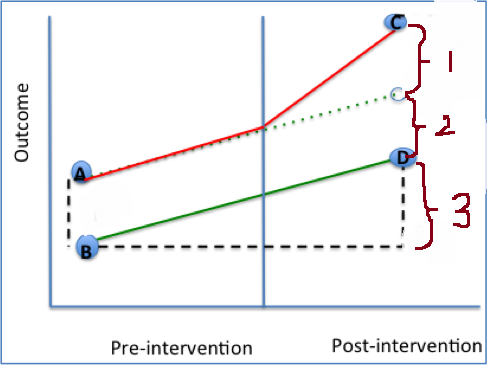
\includegraphics{"C:/Users/Claire/Dropbox/MQE_CI_Fall2020/Lecture Notes/DIDregression.png"}
\end{frame}

\end{document}
